\chapter{Các kết quả thí nghiệm}
\label{Chapter4}

\textit{Trong chương này, chúng tôi trình bày các kết quả thí nghiệm nhằm đánh giá những nội dung đã trình bày ở chương 3. Cho các thí nghiệm về nguyên lý, chúng tôi sử dụng dữ liệu được tạo ngẫu nhiên và hàm lỗi Mean Squared Error; với các thí nghiệm thực tế, chúng tôi sử dụng bộ dữ liệu MNIST và CIFAR10 và hàm lỗi Cross Entropy. Kết quả thí nghiệm cho thấy thuật toán mà chúng tôi cài đặt có thể xấp xỉ kết quả mà bài báo công bố, tuy nhiên chúng tôi nhận thấy rằng bộ siêu tham số được sử dụng để tái tạo kết quả có thể không cho kết quả tốt nhất cho tất cả thuật toán. Ngoài ra, các kết quả thí nghiệm cũng cho thấy các trường hợp mà các thuật toán khác gặp khó khăn, và cách mà Adam vượt qua các khó khăn đó. Cuối cùng, các thí nghiệm cho thấy tốc độ tối ưu hóa của các thuật toán trên các mô hình mạng nơ-ron thực tế với nhiều tầng ẩn gồm các cấu trúc khác nhau.}

\section{Các thiết lập thí nghiệm}

Chúng tôi sử dụng ngôn ngữ lập trình Python và thư viện Numpy cho các thí nghiệm nguyên lý, thư viện Pytorch cho các thí nghiệm thực tế. Cả thư viện Numpy và Pytorch đều cung cấp khả năng tăng tốc thực thi bằng việc véc-tơ hóa tính toán trên nền C/C++. Thư viện Numpy tập trung vào các chức năng tính toán đại số trên CPU, phù hợp với các thí nghiệm đơn giản; trong khi thư viện Pytorch là một thư viện máy học có thể xây dựng các mạng nơ-ron nhiều tầng ẩn phức tạp cùng với khả năng thực thi song song trên GPU. Loại GPU mà chúng tôi sử dụng là NVIDIA RTX 2080, ngoài ra chúng tôi cũng sử dụng NVIDIA Tesla T4 và Cloud Tensor Processing Unit trên nền tảng Google Colaboratory.

Trong tất cả các thí nghiệm, tất cả các thuật toán tối ưu đều có chung điểm xuất phát: bộ trọng số ban đầu đầu của mạng nơ-ron nhiều tầng ẩn sau khi khởi tạo ngẫu nhiên lần đầu sẽ được lưu lại; và với mỗi thuật toán tối ưu được thử nghiệm, bộ trọng số này sẽ được nạp lại vào mạng nơ-ron rồi từ đó mới bắt đầu tiến hành tối ưu và ghi nhận lại kết quả. Điều này giúp đảm bảo sự công bằng cho tất cả các thuật toán khi tiến hành thử nghiệm, tránh được trường hợp một thuật toán nào đó "may mắn" được bắt đầu ở một điểm thuận lợi hơn và nhờ vậy mà hội tụ nhanh hơn.

\begin{center}
	\begin{table}
		\begin{tabular}{|l|c|c|c|}
			\hline
			Tên thuật toán & Tỉ lệ học & Momentum / $Beta_1$ & Alpha / $Beta_2$ \\
			\hline
			SGD & [0.0001, 0.1] & - & - \\
			\hline
			Momentum & [0.0001, 0.1] & [0.1, 0.99] & - \\
			\hline
			Adagrad & [0.0001, 0.1] & - & - \\
			\hline
			RMSprop & [0.0001, 0.1] & - & [0.9, 0.999] \\
			\hline
			Adam & [0.0001, 0.1] & [0.1, 0.99] & [0.9, 0.999] \\
			\hline
		\end{tabular}
	\caption{\label{tab:hparam-search}Khoảng giá trị để dò tìm siêu tham số tốt nhất của các thuật toán tối ưu.}
	\end{table}
\end{center}

\section{Các kết quả thí nghiệm}

\subsection{Kết quả của thuật toán cài đặt so với bài báo}

Trong phần này, chúng tôi trình bày kết quả của các thuật toán tối ưu mà chúng tôi cài đặt. Cụ thể, chúng tôi so sánh kết quả của các thuật toán do chúng tôi cài đặt lại trên nền thư viện Pytorch với kết quả được công bố trong bài báo trong thí nghiệm Multi-layer Neural Network trên tập dữ liệu MNIST và thí nghiệm Convolutional Neural Network trên tập dữ liệu CIFAR10. Việc tái tạo các kết quả được công bố gặp nhiều khó khăn do bản chất ngẫu nhiên của SGD và dropout, cộng với việc tác giả không công bố các siêu tham số cho các thí nghiệm cũng như các cài đặt liên quan khác. Bài báo cũng không đề cập các khoảng tìm kiếm cho quá trình tìm siêu tham số tối ưu nhất của mỗi thuật toán, vì vậy chúng tôi đã tham khảo các công trình nghiên cứu khác sử dụng các tối ưu này, và tổng hợp các giá trị nhỏ nhất và lớn nhất cho từng siêu tham số của mỗi thuật toán để làm khoảng tìm kiếm (Bảng \ref{tab:hparam-search}. Bài báo thực hiện thí nghiệm với thuật toán Nesterov momentum, Adagrad, RMSprop, AdaDelta và Adam; tuy nhiên chúng tôi nhận thấy rằng Nesterov momentum và AdaDelta không liên quan trực tiếp đến thuật toán Adam mà khóa luận tập trung tìm hiểu, vì vậy chúng tôi sẽ tập trung thực hiện thí nghiệm trên các thuật toán SGD, Momentum, Adagrad, RMSprop, và Adam.

Trong thí nghiệm ``Multi-layer Neural Network'', kết quả mà chúng tôi cài đặt so với kết quả được công bố trong bài báo xấp xỉ nhau về đường đi và vị trí tương đối giữa các thuật toán với nhau (hình \ref{fig:exp-mlp}). Tuy nhiên, giá trị loss trong cài đặt của chúng tôi cũng thấp hơn đáng kể so với kết quả trong bài báo.

\begin{figure}[htp]
	\centering
	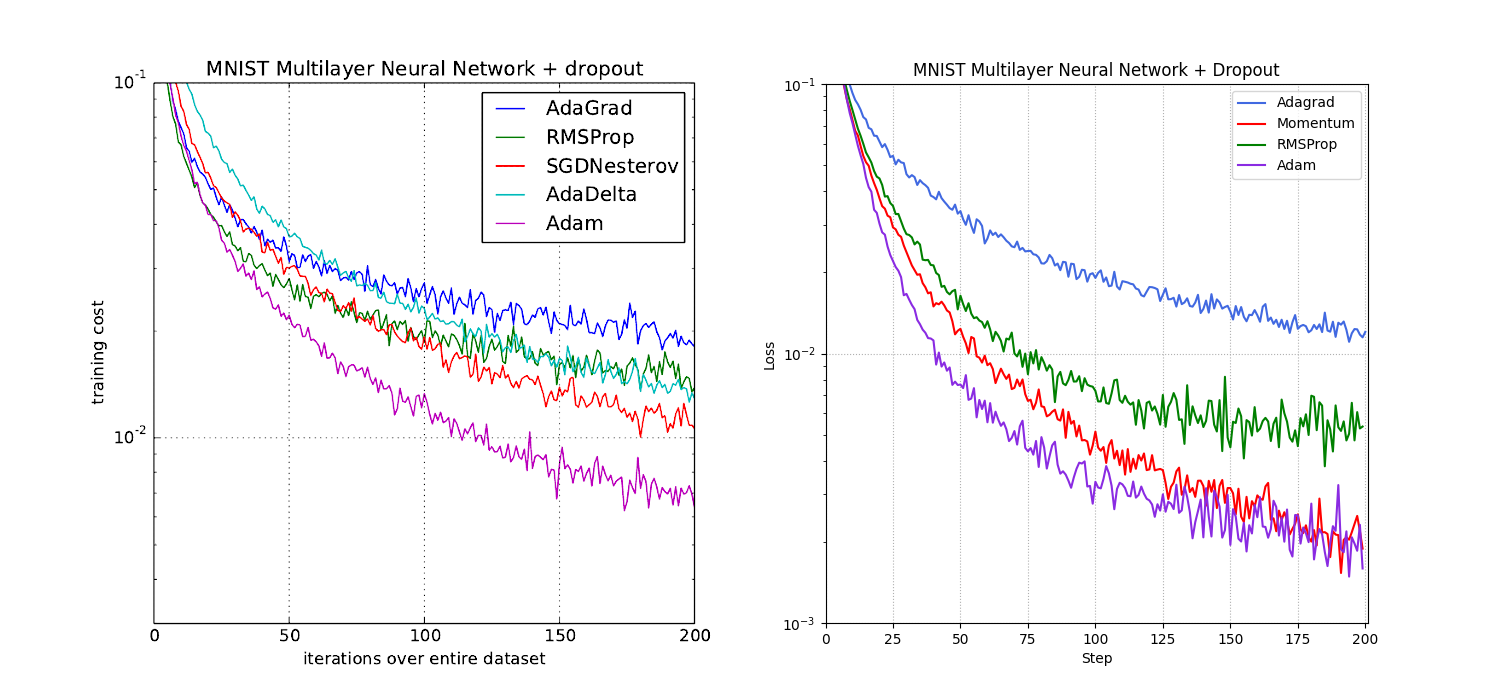
\includegraphics[width=140 mm]{images/mlp.png}
	\caption{Kết quả thí nghiệm Multi-layer Neural Network giữa thuật toán mà chúng tôi cài đặt so với bài báo. Bên trái: kết quả mà bài báo công bố. Bên phải: kết quả do chúng tôi tự cài đặt lại.}
	\label{fig:exp-mlp}
\end{figure}

Nhìn chung, thuật toán Adam có tốc độ tối ưu độ lỗi nhanh nhất trong tất cả các thuật toán được thử nghiệm. Điểm yếu của Adagrad về tỉ lệ học luôn giảm dần được thể hiện rõ khi Adagrad chuyển hướng đi ngang dần mặc dù độ lỗi vẫn cao trong khi các thuật toán khác tiếp tục đi xuống. Điều đó cho thấy rằng mô hình vẫn đang trong quá trình học dữ liệu, nhưng vì tỉ lệ học quá nhỏ nên ở mỗi bước, lượng cập nhật trọng số không đủ để cải thiện mô hình. Vấn đề tỉ lệ học giảm dần do cộng dồn gradient bình phương của Adagrad được RMSprop khắc phục bằng một tỉ lệ suy biến, giúp RMSprop bắt kịp gần hơn với Momentum và Adam. Thuật toán Momentum là thuật toán có kết quả khác biệt nhất giữa cài đặt của chúng tôi và cài đặt trong bài báo. Nếu như trong bài báo, Momentum khá xấp xỉ với RMSprop thì chúng tôi lại ghi nhận được rằng Momentum luôn luôn có độ lỗi tốt hơn RMSprop, và thậm chí còn bắt kịp với Adam ở những bước cuối cùng.

Trong thí nghiệm ``Convolutional Neural Network'', chúng tôi cũng thực hiện tìm bộ siêu tham số đem lại kết quả cuối cùng thấp nhất cho mỗi thuật toán. Tuy nhiên, sau khi đã tìm được những bộ siêu tham số cho tất cả các thuật toán và thực hiện thí nghiệm, chúng tôi thấy được rằng hầu hết các thuật toán trong cài đặt của chúng tôi đều giúp mô hình đạt được độ lỗi thấp hơn đáng kể so với bài báo khi không dùng dropout. Các giá trị siêu tham số được sử dụng được trình bày chi tiết trong bảng \ref{tab:cnn-hparam}.

Từ hình \ref{fig:exp-cnn-best}, chúng ta có thể thấy rằng bề mặt lỗi của thí nghiệm này có một đoạn dốc xuống khá rõ rệt, và các thuật toán SGD, Momentum cũng như Adam đều giảm độ lỗi rất nhanh khi tìm thấy đoạn dốc ấy. Trong bài báo gốc, một số thuật toán tìm thấy đoạn dốc này ngay từ những epoch đầu tiên, trong khi cài đặt của chúng tôi chỉ bắt đầu giảm mạnh từ khoảng epoch thứ 15. Trong kết quả của chúng tôi, SGD là thuật toán đầu tiên tìm ra đoạn dốc, nhưng độ lỗi tại epoch cuối lại hơi cao hơn so với Momentum và Adam, có thể là do SGD bị giới hạn bởi tỉ lệ học trong khi hai thuật toán kia có cơ chế tăng tốc và đạt được độ lỗi thấp.

\begin{figure}[H]
	\centering
	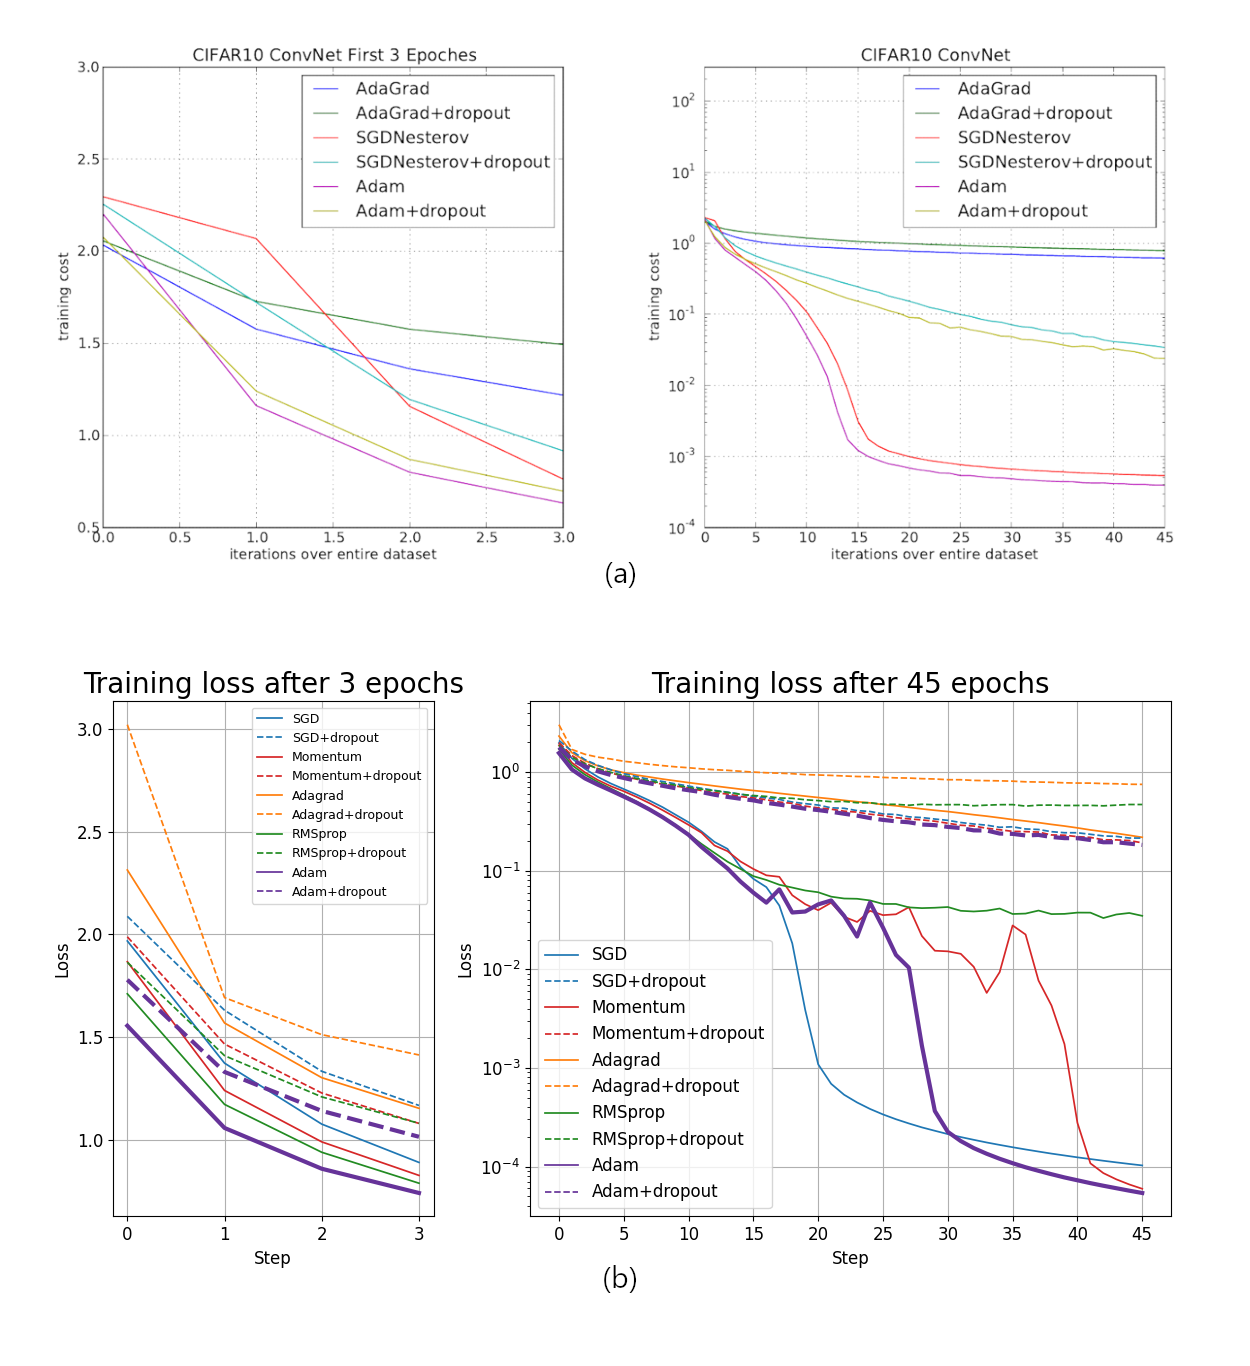
\includegraphics[width=140 mm]{images/cnn.png}
	\caption{Kết quả thí nghiệm Convolutional Neural Network giữa thuật toán mà chúng tôi cài đặt so với bài báo. (a): kết quả mà bài báo công bố. (b): kết quả do chúng tôi tự cài đặt lại.}
	\label{fig:exp-cnn-best}
\end{figure}

Ngoài việc tìm bộ siêu tham số cho kết quả tốt nhất, chúng tôi cũng cố gắng tái tạo kết quả mà bài báo đã công bố. Chúng tôi thực hiện quá trình tái tạo này để kiểm tra tính khả thi của các kết quả mà bài báo đã công bố. Hình \ref{fig:exp-cnn-rep} là kết quả sát nhất với bài báo mà chúng tôi có thể tái tạo được từ khoảng tìm kiếm mà chúng tôi sử dụng. Có thể thấy được rằng, đường đi của các thuật toán trong hình \ref{fig:exp-cnn-best}a và \ref{fig:exp-cnn-rep} có dạng khá giống nhau. Mặc dù có thể tái tạo được hình dạng biểu đồ của các thuật toán, độ lỗi cuối cùng của các thuật toán trong hình \ref{fig:exp-cnn-rep} vẫn cao hơn so với kết quả tốt nhất mà chúng tôi ghi nhận được ở hình \ref{fig:exp-cnn-best}b. Kết quả độ lỗi và thời gian thực thi được trình bày trong bảng \ref{tab:cnn-results}.

\begin{figure}[htp]
	\centering
	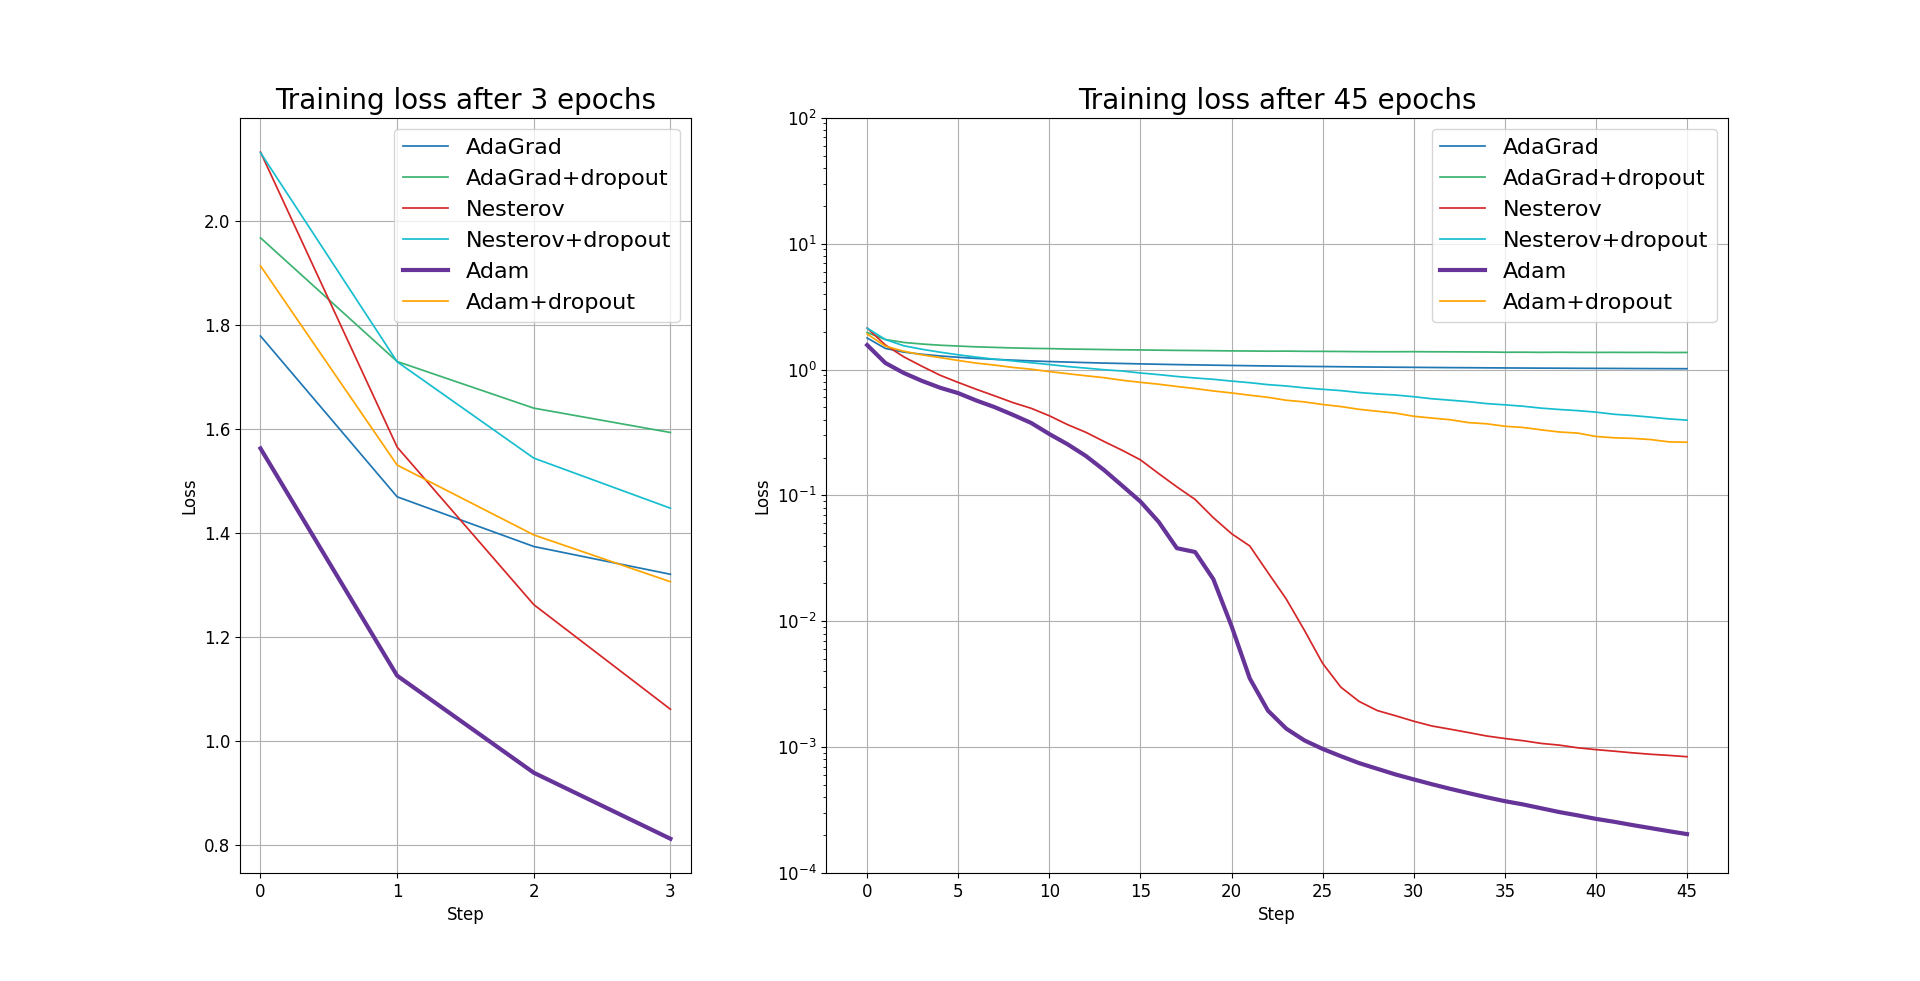
\includegraphics[width=140 mm]{images/cnn-rep.png}
	\caption{Kết quả thí nghiệm Convolutional Neural Network giữa thuật toán mà chúng tôi cài đặt với bộ siêu tham số mô phỏng kết quả của bài báo.}
	\label{fig:exp-cnn-rep}
\end{figure}

Ngoài lí do tác giả không công bố siêu tham số, cũng như tính chất ngẫu nhiên của SGD, một nguyên nhân khả thi khác cho sự khác biệt giữa kết quả mà chúng tôi ghi nhận được so với kết quả mà bài báo công bố là bản chất cài đặt của thư viện. Mỗi thư viện có cách xử lý tính toán riêng dẫn đến kết quả có phần lệch nhau. Vì tác giả cũng không nói rõ thư viện được sử dụng trong bài báo, nên thư viện Pytorch mà chúng tôi sử dụng có thể sẽ ra kết quả khác so với bài báo.

\begin{table}
	\begin{tabular}{|l|m{0.18\textwidth}|m{0.18\textwidth}|m{0.18\textwidth}|}
		\hline
		Tên thuật toán & Thời gian thực hiện (giây) & Độ lỗi thấp nhất & Độ lỗi thấp nhất (có làm trắng ảnh) \\
		\hline
		SGD                   & \textbf{6.02 $\pm $0.07} & 0.0001 & 0.0001 \\
		SGD+dropout           & \textbf{6.04 $\pm $0.07} & 0.2875 & 0.2139 \\
		\hline
		Momentum         & 6.10 $\pm$ 0.07 & \textbf{0.00007} & 0.00006 \\
		Momentum+dropout & 6.08 $\pm$ 0.07 & 0.2604 & 0.1914 \\
		\hline
		Adagrad           & 6.14 $\pm$ 0.09 & 0.2973 & 0.2178 \\
		Adagrad+dropout   & 6.16 $\pm$ 0.09 & 0.9237 & 0.7496 \\
		\hline
		RMSprop           & 6.16 $\pm$ 0.07 & 0.0395 & 0.03307 \\
		RMSprop+dropout   & 6.19 $\pm$ 0.07 & 0.4855 & 0.4512 \\
		\hline
		Adam         & 6.19$\pm$0.07 & 0.0014          & \textbf{0.000054} \\
		Adam+dropout & 6.23$\pm$0.07 & \textbf{0.2403} & \textbf{0.1824} \\
		\hline
	\end{tabular}
\caption{\label{tab:cnn-results}Kết quả và thời gian thực hiện một epoch của các thuật toán.}
\end{table}

Trong bài báo Adam, tác giả sử dụng kĩ thuật làm trắng ảnh (``whitening'') để tiền xử lý cho ảnh đầu vào. Làm trắng ảnh là quá trình tách biệt các mối liên hệ giữa các đặc trưng của ảnh, khiến các đặc trưng này trở thành độc lập\cite{kessey2015optimal}. Các đặc trưng độc lập và trùng với trục của các trọng số là một điều kiện có lợi cho các thuật toán tỉ lệ học thích ứng. Để kiểm chứng lợi thế này, chúng tôi lặp lại thí nghiệm trên, nhưng bỏ qua công đoạn làm trắng ảnh.

\begin{figure}[H]
	\centering
	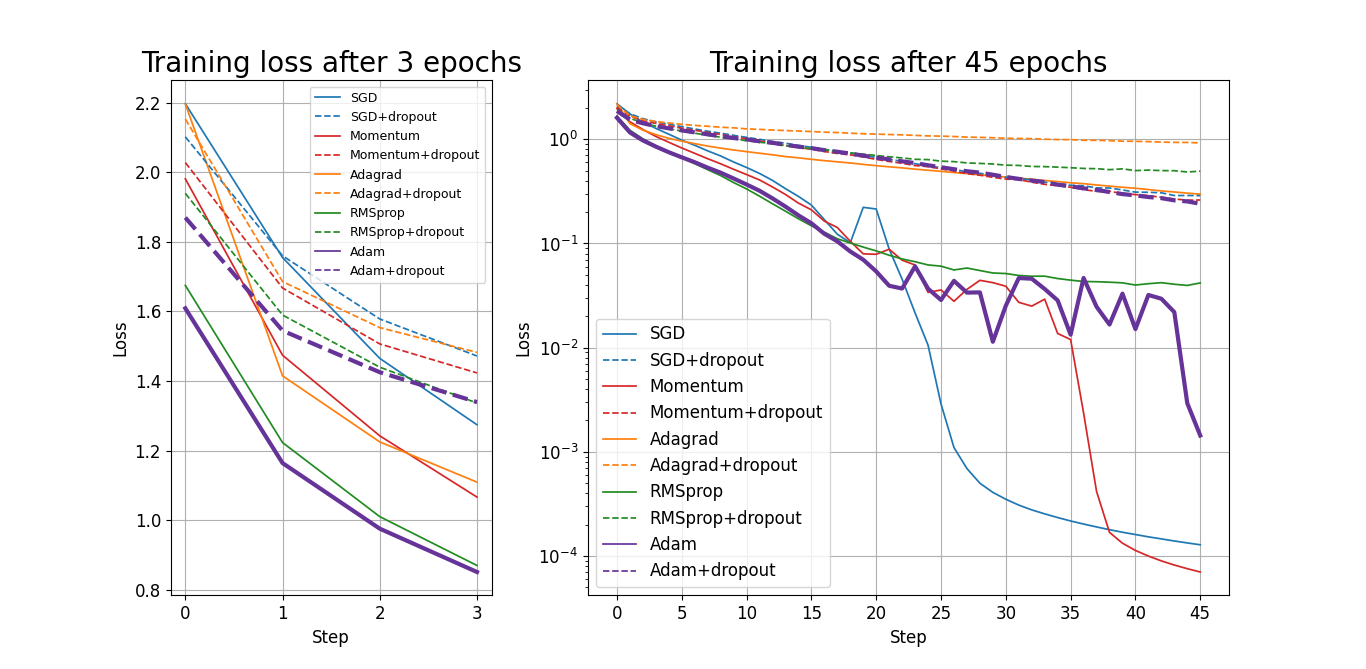
\includegraphics[width=140 mm]{images/cnn-nonwhitened.png}
	\caption{Kết quả thí nghiệm Convolutional Neural Network mà không thực hiện làm trắng ảnh.}
	\label{fig:exp-cnn-nonw}
\end{figure}

Kết quả của hình \ref{fig:exp-cnn-nonw} cho thấy độ lỗi Adam cao hơn khá nhiều khi bỏ qua bước làm trắng ảnh trong khi các thuật toán khác không bị ảnh hưởng nhiều. Như vậy, chúng ta có thể thấy việc làm trắng ảnh đầu vào sẽ giúp ích đáng kể cho quá trình huấn luyện khi sử dụng thuật toán Adam.

Về mặt thời gian tính toán, bảng \ref{tab:cnn-results} cho thấy với cùng một kích thước minibatch, có thể dễ hiểu khi SGD cho thời gian tính toán nhanh nhất vì thuật toán này chỉ tính gradient và cập nhật trọng số. Với Momentum, bước tính véc-tơ quán tính $v_t$ trước khi cập nhật trọng số làm tăng thời gian thực hiện mỗi epoch thêm khoảng 15$\%$. Bước tính đường chéo ma trận $G_t$ của các thuật toán tỉ lệ học thích ứng tốn nhiều thời gian hơn đáng kể, vì trong bước này còn có thao tác bình phương các phần tử trong véc-tơ gradient trước khi cộng dồn (thuật toán RMSprop có thêm bước nhân các phần tử này với hệ số suy biến). Adam kết hợp các bước tính quán tính trong Momentum và thích ứng tỉ lệ học, vì vậy Adam thời gian thực thi chậm nhất trong tất cả các thuật toán.

Nhìn chung, chúng tôi có thể tái tạo các kết quả thí nghiệm mà bài báo công bố. Tuy nhiên, các kết quả tốt nhất của chúng tôi có độ lỗi thấp hơn đáng kể so với bài báo, đặc biệt là trong thí nghiệm Convolutional Neural Network. Vì chúng tôi không biết chính xác quá trình cài đặt và các siêu tham số đã được sử dụng trong bài báo gốc nên chúng tôi không thể khẳng định nguyên nhân của sự chênh lệch này. Chúng tôi cũng mở rộng thí nghiệm Convolutional Neural Network để tìm hiểu ảnh hưởng của việc làm tách biệt các đặc trưng của dữ liệu thông qua thao tác làm trắng ảnh lên quá trình huấn luyện.

\subsection{Phân tích trường hợp bề mặt lỗi align và không align với tham số}

Placeholder

\subsection{Vấn đề dữ liệu thưa và nhiều lỗi}

Placeholder

\subsection{Thử nghiệm trên mô hình VGG16}

Placeholder

\subsection{Thử nghiệm trên mô hình RNN}

Placeholder